% =============================================================================
% StructureTower スーツテスト — 11 カテゴリの形式的検証
% LuaLaTeX document
% =============================================================================
\documentclass[a4paper,11pt]{ltjsarticle}

% --- Core packages ---
\usepackage{luatexja-fontspec}
\usepackage{amsmath,amssymb,amsthm}
\usepackage{mathtools}
\usepackage{tikz}
\usepackage{tikz-cd}
\usetikzlibrary{arrows.meta, positioning, shapes.geometric, fit, backgrounds, calc}
\usepackage{enumitem}
\usepackage{hyperref}
\usepackage{cleveref}
\usepackage{tcolorbox}
\usepackage{listings}
\usepackage{xcolor}
\usepackage{geometry}
\usepackage{fancyhdr}
\usepackage{float}
\usepackage{booktabs}
\usepackage{array}

% --- Page geometry ---
\geometry{margin=2.5cm, top=3cm, bottom=3cm}

% --- Fonts ---
\setmainjfont{Noto Serif JP}
\setsansjfont{Noto Sans JP}

% --- Colors ---
\definecolor{leanblue}{HTML}{2563EB}
\definecolor{leanbg}{HTML}{F8FAFC}
\definecolor{leancomment}{HTML}{6B7280}
\definecolor{leankeyword}{HTML}{7C3AED}
\definecolor{leanstring}{HTML}{059669}
\definecolor{accentcolor}{HTML}{1E40AF}
\definecolor{theoremcolor}{HTML}{EFF6FF}
\definecolor{definitioncolor}{HTML}{F0FDF4}
\definecolor{remarkcolor}{HTML}{FFF7ED}
\definecolor{countercolor}{HTML}{FEF2F2}
\definecolor{counterframe}{HTML}{DC2626}

% --- Hyperref ---
\hypersetup{
  colorlinks=true,
  linkcolor=accentcolor,
  urlcolor=leanblue,
  citecolor=accentcolor,
  pdftitle={StructureTower スーツテスト},
  pdfauthor={su},
}

% --- Theorem environments ---
\theoremstyle{definition}
\newtheorem{definition}{定義}[section]
\newtheorem{example}[definition]{例}

\theoremstyle{plain}
\newtheorem{theorem}[definition]{定理}
\newtheorem{lemma}[definition]{補題}
\newtheorem{proposition}[definition]{命題}
\newtheorem{corollary}[definition]{系}

\theoremstyle{remark}
\newtheorem{remark}[definition]{注意}
\newtheorem{counterexample}[definition]{反例}

% --- Lean code environment ---
\lstdefinelanguage{lean4}{
  morekeywords={def,theorem,lemma,example,instance,class,structure,
    where,let,in,do,if,then,else,match,with,fun,return,
    import,open,namespace,section,end,variable,
    inductive,abbrev,noncomputable,private,protected,
    sorry,admit,have,show,suffices,calc,by,exact,
    apply,intro,intros,constructor,cases,induction,
    simp,rw,rfl,ext,ring,linarith,omega,norm_num,
    decide,trivial,assumption,contradiction,
    Type,Prop,Sort,Set,true,false,
    refine,change,subst,fin_cases,
    attribute,deriving},
  sensitive=true,
  morecomment=[l]{--},
  morecomment=[n]{/-}{-/},
  morestring=[b]",
  literate=
    {α}{{\(\alpha\)}}1
    {β}{{\(\beta\)}}1
    {γ}{{\(\gamma\)}}1
    {ι}{{\(\iota\)}}1
    {ᵒᵈ}{{\(\text{}^{\mathrm{od}}\)}}2
    {→}{{\(\to\)}}1
    {←}{{\(\leftarrow\)}}1
    {↔}{{\(\leftrightarrow\)}}1
    {⟨}{{\(\langle\)}}1
    {⟩}{{\(\rangle\)}}1
    {≤}{{\(\leq\)}}1
    {≥}{{\(\geq\)}}1
    {≠}{{\(\neq\)}}1
    {∀}{{\(\forall\)}}1
    {∃}{{\(\exists\)}}1
    {∧}{{\(\wedge\)}}1
    {∨}{{\(\vee\)}}1
    {¬}{{\(\neg\)}}1
    {⊢}{{\(\vdash\)}}1
    {∈}{{\(\in\)}}1
    {∉}{{\(\notin\)}}1
    {⊆}{{\(\subseteq\)}}1
    {∪}{{\(\cup\)}}1
    {∩}{{\(\cap\)}}1
    {∅}{{\(\emptyset\)}}1
    {ℕ}{{\(\mathbb{N}\)}}1
    {ℤ}{{\(\mathbb{Z}\)}}1
    {ℝ}{{\(\mathbb{R}\)}}1
    {:=}{{:=}}2,
}

\lstnewenvironment{leancode}[1][]{%
  \lstset{
    language=lean4,
    basicstyle=\ttfamily\small,
    keywordstyle=\color{leankeyword}\bfseries,
    commentstyle=\color{leancomment}\itshape,
    stringstyle=\color{leanstring},
    backgroundcolor=\color{leanbg},
    frame=single,
    rulecolor=\color{leanblue!30},
    framesep=8pt,
    xleftmargin=12pt,
    xrightmargin=12pt,
    breaklines=true,
    breakatwhitespace=true,
    showstringspaces=false,
    tabsize=2,
    captionpos=b,
    numbers=left,
    numberstyle=\tiny\color{leancomment},
    numbersep=8pt,
    aboveskip=1em,
    belowskip=1em,
    #1
  }%
}{}

% --- Tcolorbox styles ---
\newtcolorbox{proofstrategy}{
  colback=remarkcolor,
  colframe=orange!60!black,
  title={\textbf{証明戦略}},
  fonttitle=\sffamily,
  boxrule=0.5pt,
  arc=3pt,
}

\newtcolorbox{mathinsight}{
  colback=theoremcolor,
  colframe=accentcolor,
  title={\textbf{数学的洞察}},
  fonttitle=\sffamily,
  boxrule=0.5pt,
  arc=3pt,
}

\newtcolorbox{counterpointbox}{
  colback=countercolor,
  colframe=counterframe,
  title={\textbf{反例・注意点}},
  fonttitle=\sffamily,
  boxrule=0.5pt,
  arc=3pt,
}

% --- Header/Footer ---
\pagestyle{fancy}
\fancyhf{}
\renewcommand{\headrulewidth}{0.4pt}
\fancyhead[L]{\small\sffamily\nouppercase{\leftmark}}
\fancyhead[R]{\small\sffamily StructureTower スーツテスト}
\fancyfoot[C]{\thepage}

% --- Math macros ---
\newcommand{\ST}{\mathsf{ST}}    % StructureTower の略記
\newcommand{\ET}{\mathsf{ET}}    % ExhaustiveTower の略記
\newcommand{\lev}{\mathrm{level}}
\newcommand{\union}{\mathrm{union}}
\newcommand{\glob}{\mathrm{global}}
\newcommand{\rank}{\mathrm{rank}}
\newcommand{\op}{\mathrm{op}}

% =============================================================================
\begin{document}

\title{%
  {\LARGE\sffamily\bfseries StructureTower スーツテスト}\\[0.5em]
  {\large\sffamily Lean 4 による 11 カテゴリの形式的検証}%
}
\author{su}
\date{\today}
\maketitle

\begin{center}
\small
\textit{AI assistance disclosure:}\\
Lean ソースコードは Claude (Anthropic) で課題を生成し、
Codex (OpenAI) で生成した。\\
\TeX\ 文書は Claude Code (Anthropic) で生成した。\\
著者による加筆・修正は行っていない。\\
内容の正確性は保証されず、誤りがあれば著者の責任である。
\end{center}

\vspace{1em}

\begin{abstract}
本稿は Lean 4 / Mathlib4 で形式化された \texttt{StructureTower} フレームワークの
「スーツテスト（Suit Tests）」を数学的に解説する。
スーツテストとは、抽象的な定義に対して \textbf{11 のカテゴリ}から具体例・反例・
境界事例を系統的に与えることで、定義の整合性と Lean 実装の健全性を確認する
検証スイートである。
対象となる主要構造は、前順序 $\iota$ で添字付けられた単調集合族
$\{T_i\}_{i \in \iota}$（\emph{構造塔}、以下 $\ST\,\iota\,\alpha$ と記す）と、
それを拡張した \emph{網羅的塔}（$\ET\,\iota\,\alpha$）および
\emph{特性ランク}（CharRank）である。
本文では各テストカテゴリの数学的意義を解説し、
Lean による証明の戦略を説明する。
\end{abstract}

\tableofcontents
\newpage

% =============================================================================
\section{はじめに}\label{sec:intro}
% =============================================================================

\subsection{StructureTower とは}

\emph{構造塔}（StructureTower）は、Bourbaki の母構造論からインスピレーションを
得た概念であり、前順序集合 $\iota$ で添字付けられた集合族
$T = \{\lev_T(i)\}_{i \in \iota}$（各 $\lev_T(i) \subseteq \alpha$）であって、
\[
  i \leq j \implies \lev_T(i) \subseteq \lev_T(j)
\]
という単調性条件を満たすものである。
直観的には、「大きい添字の層にはより多くの要素が含まれる」という
フィルトレーション（濾過）構造を抽象化している。

\begin{figure}[H]
\centering
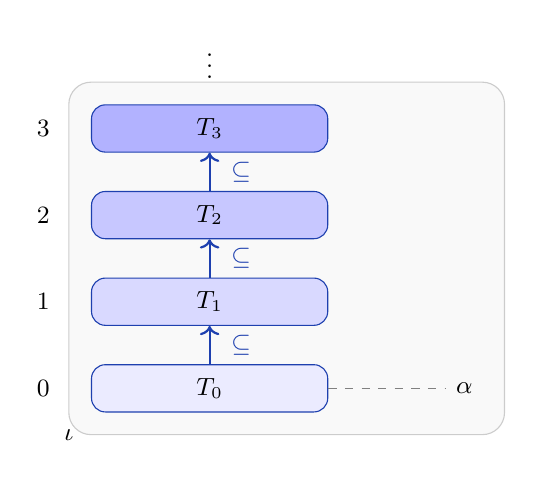
\begin{tikzpicture}[
  layer/.style={rectangle, rounded corners=5pt, draw=accentcolor, fill=theoremcolor,
                minimum width=3cm, minimum height=0.6cm, font=\small},
  every node/.style={font=\small}
]
  \node[layer, fill=blue!8]  (L0) at (0,0)   {$T_0$};
  \node[layer, fill=blue!15] (L1) at (0,1.1) {$T_1$};
  \node[layer, fill=blue!22] (L2) at (0,2.2) {$T_2$};
  \node[layer, fill=blue!30] (L3) at (0,3.3) {$T_3$};
  \node at (0,4.2) {$\vdots$};

  \draw[->, thick, accentcolor] (L0.north) -- (L1.south)
        node[midway, right=4pt] {$\subseteq$};
  \draw[->, thick, accentcolor] (L1.north) -- (L2.south)
        node[midway, right=4pt] {$\subseteq$};
  \draw[->, thick, accentcolor] (L2.north) -- (L3.south)
        node[midway, right=4pt] {$\subseteq$};

  \node[right=1.5cm of L0] (alpha0) {$\alpha$};
  \draw[dashed, gray] (L0.east) -- (alpha0);

  \begin{scope}[on background layer]
    \node[draw=gray!40, fill=gray!5, rounded corners=8pt,
          fit=(L0)(L3)(alpha0), inner sep=8pt] {};
  \end{scope}

  \node[left=0.4cm of L0] {$0$};
  \node[left=0.4cm of L1] {$1$};
  \node[left=0.4cm of L2] {$2$};
  \node[left=0.4cm of L3] {$3$};
  \node[left=0.3cm of L0, yshift=-0.6cm, xshift=0.2cm] {$\iota$};
\end{tikzpicture}
\caption{構造塔の概念図。添字 $i \in \iota$ が大きくなるにつれ、
  層 $\lev_T(i) \subseteq \alpha$ が単調に拡大する。}
\label{fig:tower-concept}
\end{figure}

\subsection{スーツテストの目的と 11 カテゴリ}

「スーツテスト」とは、定義の健全性を多角的に検証するための
体系的なテストスイートである。
各カテゴリに名前が付いており、どのような性質を試験するかが明確になっている。
11 のカテゴリを表~\ref{tab:suit-categories} に示す。

\begin{table}[H]
\centering
\caption{11 カテゴリのスーツテスト一覧}\label{tab:suit-categories}
\begin{tabular}{rlll}
\toprule
\# & スーツ名 & 日本語 & 主要な内容 \\
\midrule
P1  & trivial              & 自明例     & \texttt{emptyTower}（空集合・空虚真） \\
P2  & canonical            & 標準例     & \texttt{natExhaustive}, \texttt{HasCharRank}, ランク一意性 \\
P3  & extreme              & 極端例     & 順序数 $\omega_0$-有界塔 \\
P4  & pathological         & 病的例     & \texttt{FakeTower}（単調性の失敗） \\
P5  & counterexample       & 反例       & \texttt{TwoPoint}（前順序でのランク非一意性） \\
P6  & dual                 & 双対例     & \texttt{idealPowTower}（双対順序・イデアル冪） \\
P7  & borderline           & 境界例     & シングルトン族の失敗・\texttt{natFiltration} 層分解 \\
P8  & non-example          & 非例       & \texttt{almostFiltered}（単調だが加法非閉） \\
P9  & out-of-category      & 圏外例     & 最終的単調列と打ち切り \\
P10 & schema               & スキーマ   & \texttt{thresholdTower}（重み関数による塔の生成） \\
P11 & finite-computational & 有限計算例 & \texttt{finTower1}/\texttt{finTower2}（Fin 3 × Fin 5） \\
\bottomrule
\multicolumn{4}{l}{\small ※ 本文の基本定義節（§\ref{sec:basic}）は各 P に先立つインフラ定義を解説する。}
\end{tabular}
\end{table}

% =============================================================================
\section{基本定義}\label{sec:defs}
% =============================================================================

\begin{definition}[StructureTower]\label{def:structure-tower}
$\iota, \alpha$ を型とし、$\iota$ 上に前順序 $\leq$ が与えられているとする。
\emph{構造塔} $T$（型 $\ST\,\iota\,\alpha$）とは、以下のデータからなる構造体である：
\begin{itemize}
  \item 層関数 $\lev_T : \iota \to \mathcal{P}(\alpha)$（$\mathcal{P}$ は冪集合）
  \item 単調性：$\forall i, j \in \iota,\; i \leq j \implies \lev_T(i) \subseteq \lev_T(j)$
\end{itemize}
\end{definition}

\begin{definition}[union, global]\label{def:union-global}
構造塔 $T : \ST\,\iota\,\alpha$ に対し：
\[
  \union(T) := \bigcup_{i \in \iota} \lev_T(i), \qquad
  \glob(T) := \bigcap_{i \in \iota} \lev_T(i).
\]
\end{definition}

\begin{definition}[ExhaustiveTower]\label{def:exhaustive}
$\iota$ を前順序型，$\alpha$ を型とする。
$T : \ST\,\iota\,\alpha$ が \emph{網羅的} であるとは，
\[
  \forall x \in \alpha,\; \exists i \in \iota,\; x \in \lev_T(i)
\]
が成り立つことをいう。このとき $T$ を
$\ET\,\iota\,\alpha$（ExhaustiveTower）と呼ぶ。

\begin{remark}
添字型 $\iota$ は任意の前順序でよい（$\iota = \mathbb{N}$ に限らない）。
例えば，後述する \texttt{twoPointExhaustive} は
$\ET\,\mathsf{TwoPoint}\,\mathbb{N}$ の元である。
\emph{ランク関数}（rank）は $\iota = \mathbb{N}$ の場合のみ
\texttt{Nat.find} により構成できる。
\end{remark}
\end{definition}

\begin{definition}[HasCharRank --- $\mathbb{N}$-添字版]\label{def:charrank}
$T : \ET\,\mathbb{N}\,\alpha$，$r : \alpha \to \mathbb{N}$ とする。
$r$ が $T$ の \emph{特性ランク関数}（HasCharRank）であるとは：
\[
  \forall x \in \alpha,\, \forall n \in \mathbb{N},\quad
  x \in \lev_T(n) \iff r(x) \leq n.
\]
\end{definition}

\begin{definition}[HasCharRankPreorder --- 一般前順序版]\label{def:charrank-preorder}
$\iota$ を前順序型，$T : \ET\,\iota\,\alpha$，$r : \alpha \to \iota$ とする。
$r$ が $T$ の \emph{前順序特性ランク関数}（HasCharRankPreorder）であるとは：
\[
  \forall x \in \alpha,\, \forall i \in \iota,\quad
  x \in \lev_T(i) \iff r(x) \leq i.
\]

\begin{remark}
定義~\ref{def:charrank} は $\iota = \mathbb{N}$ の特殊ケースに相当する。
$\iota = \mathbb{N}$（部分順序）では HasCharRank が一意だが，
一般の前順序では一意性が崩れる（§\ref{sec:preorder} 参照）。
\end{remark}
\end{definition}

% =============================================================================
\section{インフラ：基本的な塔の構成}\label{sec:basic}
% =============================================================================

\subsection{下切り塔 \texttt{iic}}

\begin{definition}[下切り塔]\label{def:iic}
前順序集合 $\alpha$ に対し，\emph{下切り塔} $\mathsf{iic}(\alpha) : \ST\,\alpha\,\alpha$ を
\[
  \lev_{\mathsf{iic}}(x) := \{y \in \alpha \mid y \leq x\} = (-\infty, x]
\]
で定義する。
特殊ケース $\mathsf{natFiltration} := \mathsf{iic}(\mathbb{N})$（自然数フィルトレーション）が
標準例 P2 の基礎となる。
\end{definition}

\begin{proposition}
$\mathsf{iic}(\alpha)$ は単調性条件を満たす。
\end{proposition}
\begin{proof}
$z \leq x$ かつ $x \leq y$ なら，推移律より $z \leq y$。
\end{proof}

\begin{leancode}[caption={iic と natFiltration の定義}]
def iic (α : Type*) [Preorder α] : StructureTower α α where
  level x := Set.Iic x
  monotone_level := by
    intro i j hij x hx
    exact le_trans hx hij

def natFiltration : StructureTower ℕ ℕ := iic ℕ
\end{leancode}

\subsection{反変族から塔を構成する \texttt{ofAntitone}}

自然な順序に関して単調減少する集合族（反変族）からも構造塔が作れる。
鍵となるのは \emph{双対順序}（order dual）$\iota^{\op}$ の利用である。

\begin{definition}[ofAntitone]\label{def:ofantitone}
$d : \iota \to \mathcal{P}(\alpha)$ が反変（$i \leq j \implies d(j) \subseteq d(i)$）
であるとき，$\mathsf{ofAntitone}(d) : \ST\,\iota^{\op}\,\alpha$ を
$\lev(i) := d(\bar{i})$（$\bar{i}$ は双対順序における像）で定義する。
\end{definition}

\begin{figure}[H]
\centering
\begin{tikzcd}[column sep=large]
  \iota^{\op}
    \arrow[r, "\lev", "{\mathsf{ofAntitone}(d)}"']
    \arrow[d, "\overline{(\cdot)}"']
  & \mathcal{P}(\alpha) \\
  \iota
    \arrow[ur, "d"']
\end{tikzcd}
\caption{\texttt{ofAntitone} の可換図式。
  双対順序 $\iota^{\op}$ 上では単調，元の順序 $\iota$ 上では反変。}
\label{fig:ofantitone}
\end{figure}

\begin{leancode}[caption={ofAntitone の定義（双対順序を活用）}]
def ofAntitone {ι α : Type*} [Preorder ι] (d : ι → Set α) (hd : Antitone d) :
    StructureTower ιᵒᵈ α where
  level i := d (OrderDual.ofDual i)
  monotone_level := by
    intro i j hij x hx
    exact hd (OrderDual.ofDual_le_ofDual.mpr hij) hx
\end{leancode}

\subsection{交差塔 \texttt{inter}}

\begin{definition}[交差塔]\label{def:inter}
$T_1, T_2 : \ST\,\iota\,\alpha$ に対し，
$(T_1 \cap T_2)_i := \lev_{T_1}(i) \cap \lev_{T_2}(i)$
と定義される $\mathsf{inter}(T_1, T_2) : \ST\,\iota\,\alpha$ を \emph{交差塔} と呼ぶ。
\end{definition}

\begin{proposition}
交差塔は単調性を満たす。
\end{proposition}
\begin{proof}
$i \leq j$ のとき，$T_1, T_2$ それぞれの単調性から
$(T_1 \cap T_2)_i \subseteq (T_1 \cap T_2)_j$。
\end{proof}

% =============================================================================
\section{P1（trivial）：空の塔}\label{sec:empty}
% =============================================================================

\begin{example}[空の塔]\label{ex:empty}
$\alpha = \mathsf{Empty}$（空型），$\iota = \mathsf{Unit}$（1点型）として，
$\lev_{\mathsf{emptyTower}}(\star) := \emptyset$
と定義する。
空集合は任意の集合に包含されるので単調性は自明に成立する。
特に $\union(\mathsf{emptyTower}) = \emptyset$。
\end{example}

\begin{mathinsight}
空の塔は「最小の塔」の役割を果たす。
Lean では空型 \texttt{Empty} の要素は存在しないため，
単調性の証明は \texttt{cases hx} で即座に終わる。
これは \emph{空虚真}（vacuous truth）の実装例である。
\end{mathinsight}

\begin{leancode}[caption={空の塔と基本定理（P1: trivial）}]
def emptyTower : StructureTower Unit Empty where
  level := fun _ => ∅
  monotone_level := by
    intro i j hij x hx
    cases hx  -- Empty 型なので hx は矛盾

theorem emptyTower_union_eq :
    emptyTower.union = ∅ := by
  ext x; cases x  -- Empty 型に要素なし
\end{leancode}

% =============================================================================
\section{P2（canonical）：網羅的塔とランク}\label{sec:exhaustive}
% =============================================================================

\subsection{自然数フィルトレーションの網羅性}

\begin{proposition}
$\mathsf{natExhaustive} := \mathsf{iic}(\mathbb{N})$ は $\ET\,\mathbb{N}\,\mathbb{N}$ の元であり，
恒等写像 $r = \mathrm{id}_\mathbb{N}$ が特性ランク関数となる。
\end{proposition}
\begin{proof}
任意の $x \in \mathbb{N}$ に対し $x \in \lev_x$（$x \leq x$）なので網羅的。
ランクについては $x \in \lev_n \iff x \leq n \iff \mathrm{id}(x) \leq n$。
\end{proof}

\begin{theorem}[ランク一意性（$\mathbb{N}$-添字の場合）]\label{thm:rank-unique}
$T : \ET\,\mathbb{N}\,\alpha$ において，
特性ランク関数は一意である：
\[
  \mathsf{HasCharRank}(T, r_1) \wedge \mathsf{HasCharRank}(T, r_2) \implies r_1 = r_2.
\]
\end{theorem}

\begin{mathinsight}
証明の核心：任意の $x$ に対し，CharRank の条件から
$r_1(x) \leq r_2(x)$ かつ $r_2(x) \leq r_1(x)$。
$\mathbb{N}$ の反対称律（\texttt{Nat.le\_antisymm}）から $r_1(x) = r_2(x)$。
なお $\mathbb{N}$ は常に部分順序であるため，
「添字型が部分順序である」という条件は自明に成立する。
一般の前順序 $\iota$ では反対称律がなく，この結論は成立しない（P5 参照）。
\end{mathinsight}

\begin{leancode}[caption={natExhaustive の定義とランク等式（P2: canonical）}]
def natExhaustive : ExhaustiveTower ℕ ℕ where
  toStructureTower := natFiltration
  exhaustive := by
    intro x
    refine ⟨x, ?_⟩
    change x ≤ x
    exact le_rfl

theorem natExhaustive_rank_eq (x : ℕ) :
    natExhaustive.rank x = x := by
  have h := congrFun (rank_unique natExhaustive id
                        natExhaustive_hasCharRank) x
  simpa using h.symm
\end{leancode}

% =============================================================================
\section{P3（extreme）：順序数による塔}\label{sec:ordinal}
% =============================================================================

\subsection{$\omega_0$-有界順序数による自然数の塔}

\begin{definition}[ordinalNatBound]
$o < \omega_0$（最初の極限順序数）のとき，$o$ に対応する自然数
$\mathsf{ordinalNatBound}(o) \in \mathbb{N}$ を，
$o = \overline{n}$（$n \in \mathbb{N}$ の順序数へのキャスト）
となる $n$ の古典的選択（\texttt{Classical.choose}）で定める。

\begin{remark}
Lean 4 Mathlib（v4.28.0 時点）には \texttt{Ordinal.toNat} は存在しない。
直接 \texttt{Ordinal.lt\_omega0.mp} と \texttt{Classical.choose} を組み合わせる
必要がある。これが \texttt{noncomputable} を要する理由である。
\end{remark}
\end{definition}

\begin{definition}[ordinalTower]
$\mathsf{ordinalTower} : \ST\,\mathsf{Ord}\,\mathbb{N}$ を
\[
  \lev(o) :=
  \begin{cases}
    \{n \in \mathbb{N} \mid n \leq \mathsf{ordinalNatBound}(o)\} & (o < \omega_0) \\
    \mathbb{N} & (o \geq \omega_0)
  \end{cases}
\]
で定義する。
\end{definition}

\begin{figure}[H]
\centering
\begin{tikzpicture}[scale=0.9,
  every node/.style={font=\small}
]
  \draw[->] (-0.5,0) -- (7,0) node[right] {順序数 $o$};
  \foreach \x/\lab in {0/$0$, 1/$1$, 2/$2$, 3/$3$, 4/$\cdots$, 5/$\omega_0$, 6/$\omega_0\!+\!1$}
    \node[below] at (\x, -0.1) {\lab};
  \foreach \x in {0,1,2,3,5,6}
    \draw (\x, -0.05) -- (\x, 0.05);

  \foreach \x/\h/\col in {
    0/0.4/blue!15,
    1/0.7/blue!20,
    2/1.0/blue!25,
    3/1.3/blue!30,
    5/2.0/blue!50,
    6/2.0/blue!50}
  {
    \fill[\col] (\x-0.35, 0.1) rectangle (\x+0.35, \h);
    \draw[blue!60] (\x-0.35, 0.1) rectangle (\x+0.35, \h);
  }
  \node[right=6pt] at (6, 1.0) {$= \mathbb{N}$};

  \node[above] at (0, 0.4)  {\tiny $\{0\}$};
  \node[above] at (1, 0.7)  {\tiny $\{0,1\}$};
  \node[above] at (2, 1.0)  {\tiny $\{0,1,2\}$};

  \draw[dashed, gray] (4.6, 0) -- (4.6, 2.2);
  \node[above] at (4.8, 2.0) {\scriptsize $\omega_0$ の壁};
\end{tikzpicture}
\caption{\texttt{ordinalTower} の層。$o < \omega_0$ では有限層，$o \geq \omega_0$ では $\mathbb{N}$ 全体。
  和集合は $\mathbb{N}$ に等しい（\texttt{Ordinal.nat\_lt\_omega0} を使用）。}
\label{fig:ordinal-tower}
\end{figure}

\begin{theorem}
$\union(\mathsf{ordinalTower}) = \mathbb{N}$。
\end{theorem}
\begin{proof}
任意の $x \in \mathbb{N}$ に対し，Mathlib の補題
\texttt{Ordinal.nat\_lt\_omega0} より $\overline{x} < \omega_0$。
よって $\mathsf{ordinalNatBound}(\overline{x}) = x$ が確認でき，
$x \in \lev(\overline{x})$。
\end{proof}

% =============================================================================
\section{P4（pathological）：反例 — 単調性の失敗}\label{sec:fake}
% =============================================================================

\begin{counterexample}[\texttt{fakeExample}]\label{ex:fake}
$\mathbb{N}$ 上の集合族
\[
  S_n :=
  \begin{cases}
    \{0, 1\} & (n = 0) \\
    \{2\}    & (n \geq 1)
  \end{cases}
\]
は単調でない：$S_0 = \{0,1\} \not\subseteq \{2\} = S_1$（$0 \in S_0$ だが $0 \notin S_1$）。
\end{counterexample}

\begin{counterpointbox}
\texttt{FakeTower} は \texttt{monotone\_level} フィールドを持たない
``偽の塔'' 構造体であり，単調性公理の不可欠性を示す。
Lean での証明は：$S_0 \subseteq S_1$ を仮定すると $0 \in S_1 = \{2\}$ となり
矛盾（\texttt{simp} で自動解決）。
\end{counterpointbox}

% =============================================================================
\section{P5（counterexample）：前順序でのランク非一意性}\label{sec:preorder}
% =============================================================================

\subsection{二点前順序}

\begin{definition}[TwoPoint 前順序]\label{def:twopoint}
集合 $\{a, b\}$（$a \neq b$）上に，
$x \leq y$ が全ての対で成立する前順序（全関係）を与える：
\[
  a \leq b \quad \text{かつ} \quad b \leq a \quad \text{だが} \quad a \neq b.
\]
これは反対称律（$x \leq y \wedge y \leq x \Rightarrow x = y$）が成立しない前順序の最小例である。
\end{definition}

\begin{theorem}[前順序ではランクが非一意]\label{thm:rank-not-unique}
$\mathsf{twoPointExhaustive}$（全層が $\mathbb{N}$ である $\ET\,\mathsf{TwoPoint}\,\mathbb{N}$）に対し，
定数関数 $r_1 \equiv a$ および $r_2 \equiv b$ はいずれも
HasCharRankPreorder を満たすが $r_1 \neq r_2$ である。
\end{theorem}

\begin{figure}[H]
\centering
\begin{tikzpicture}[every node/.style={font=\small}]
  % TwoPoint preorder diagram
  \node[draw, circle, minimum size=0.8cm, fill=orange!20] (a) at (-1, 0) {$a$};
  \node[draw, circle, minimum size=0.8cm, fill=orange!20] (b) at (1, 0)  {$b$};
  \draw[->, bend left=25, thick] (a) to node[above] {$\leq$} (b);
  \draw[->, bend left=25, thick] (b) to node[below] {$\leq$} (a);
  \node[below=0.5cm] at (0, -0.4) {\small $a \neq b$ だが $a \leq b \leq a$};

  % Rank maps
  \node (N) at (-4, 0) {$\mathbb{N}$};
  \draw[->, bend left=20, accentcolor, thick] (N) to node[above left] {$r_1 \equiv a$} (a);
  \draw[->, bend right=20, accentcolor!60, thick] (N) to node[below left] {$r_2 \equiv b$} (b);
\end{tikzpicture}
\caption{二点前順序 $\{a,b\}$ と二つのランク写像。
  $a \leq b \leq a$ だが $a \neq b$ なので反対称律が成立せず，
  ランク一意性が崩れる。}
\label{fig:rank-nonunique}
\end{figure}

\begin{mathinsight}
定理~\ref{thm:rank-unique} が成立するのは添字型が
$\mathbb{N}$（部分順序）のときである。
前順序では $r_1(x) \leq r_2(x)$ かつ $r_2(x) \leq r_1(x)$ から
$r_1(x) = r_2(x)$ が導けない（反対称律なし）。
この反例では $a \leq b \leq a$ かつ $a \neq b$ がまさにそのケースを実現する。
\end{mathinsight}

\begin{leancode}[caption={rank 非一意性の証明（P5: counterexample）}]
theorem rank_not_unique_preorder :
    ∃ (r₁ r₂ : ℕ → TwoPoint), r₁ ≠ r₂ ∧
      HasCharRankPreorder twoPointExhaustive r₁ ∧
      HasCharRankPreorder twoPointExhaustive r₂ := by
  refine ⟨twoPointRankA, twoPointRankB, ?_,
          twoPointRankA_hasChar, twoPointRankB_hasChar⟩
  intro h
  -- r₁ = r₂ を仮定すると congrFun で a = b
  have : TwoPoint.a = TwoPoint.b := congrFun h 0
  cases this   -- TwoPoint.a ≠ TwoPoint.b（DecidableEq）
\end{leancode}

% =============================================================================
\section{P6（dual）：双対順序とイデアル冪}\label{sec:ideal}
% =============================================================================

\subsection{可換環のイデアル冪列}

\begin{definition}[idealPowTower]\label{def:ideal-pow}
可換環 $R$ のイデアル $I \trianglelefteq R$ に対し，
$n \mapsto I^n$ は \emph{反変}：
\[
  m \leq n \implies I^n \subseteq I^m.
\]
双対順序 $\mathbb{N}^{\op}$ を添字として
$\mathsf{idealPowTower}(I) : \ST\,\mathbb{N}^{\op}\,R$，
$\lev(n) := I^n$ を得る。
\end{definition}

\begin{figure}[H]
\centering
\begin{tikzpicture}[
  every node/.style={font=\small}
]
  \node at (-1.5, 2) {$\mathbb{N}$（通常順序）};
  \foreach \n in {0,1,2,3}
    \node[draw, circle, minimum size=0.6cm, fill=blue!10]
      (N\n) at (-3 + \n*0.9, 0.5) {\n};
  \draw[->] (N0) -- (N1);
  \draw[->] (N1) -- (N2);
  \draw[->] (N2) -- (N3);
  \node at (-3+3.5*0.9, 0.5) {$\cdots$};

  \node at (3, 2) {$\mathbb{N}^{\op}$（双対順序）};
  \foreach \n in {0,1,2,3}
    \node[draw, circle, minimum size=0.6cm, fill=orange!20]
      (M\n) at (1.5 + \n*0.9, 0.5) {\n};
  \draw[<-] (M0) -- (M1);
  \draw[<-] (M1) -- (M2);
  \draw[<-] (M2) -- (M3);
  \node at (1.5+3.5*0.9, 0.5) {$\cdots$};

  \node at (3, -0.8) {$I^0 \supseteq I^1 \supseteq I^2 \supseteq \cdots$};
  \foreach \n in {0,1,2,3}
    \draw[->, dashed, gray] (M\n) -- (1.5+\n*0.9, -0.5);
\end{tikzpicture}
\caption{イデアル冪塔の構造（P6: dual）。
  通常 $\mathbb{N}$ 上では反変なので，
  双対順序 $\mathbb{N}^{\op}$ を添字にすることで構造塔を得る。}
\label{fig:ideal-pow}
\end{figure}

\begin{proposition}
$\mathsf{idealPowTower}(I) = \mathsf{ofAntitone}(\mathsf{idealPowAntitone}(I))$。
\end{proposition}
\begin{proof}
$\lev$ の定義を展開すると両辺が一致する（\texttt{ext} + \texttt{simp}）。
\end{proof}

\begin{leancode}[caption={idealPowTower の定義（P6: dual）}]
noncomputable def idealPowTower (I : Ideal R) : StructureTower ℕᵒᵈ R where
  level n := ↑(I ^ OrderDual.ofDual n)
  monotone_level := by
    intro i j hij x hx
    exact (Ideal.pow_le_pow_right (I := I)
      (m := OrderDual.ofDual j) (n := OrderDual.ofDual i)
      (OrderDual.ofDual_le_ofDual.mpr hij)) hx
\end{leancode}

% =============================================================================
\section{P7（borderline）：シングルトンと層分解}\label{sec:singleton}
% =============================================================================

\subsection{シングルトン族は塔にならない}

\begin{counterexample}[\texttt{singletonTowerFails}]
$S_n := \{n\}$（シングルトン族）は単調でない：
$n < m$ に対し $n \in S_n$ だが $n \notin S_m = \{m\}$。
よって $\mathsf{StructureTower}$ を構成できない（境界例：単調性がほぼ成立するが失敗）。
\end{counterexample}

\subsection{natFiltration の層分解}

\begin{proposition}[層分解定理]\label{prop:layer}
$n \geq 1$ のとき：
\[
  \lev_n \setminus \lev_{n-1} = \{n\}.
\]
各層は厚み 1 の「殻」を積み上げた構造を持つ。
\end{proposition}

\begin{figure}[H]
\centering
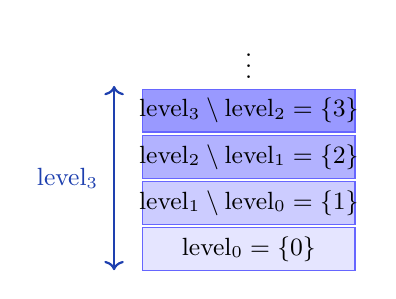
\begin{tikzpicture}[scale=0.9, every node/.style={font=\small}]
  \foreach \n/\col in {
    0/blue!10,
    1/blue!20,
    2/blue!30,
    3/blue!40}
  {
    \fill[\col] (0, \n*0.65) rectangle (3, \n*0.65+0.6);
    \draw[blue!60] (0, \n*0.65) rectangle (3, \n*0.65+0.6);
  }
  \node at (1.5, 0*0.65+0.3) {$\lev_0 = \{0\}$};
  \node at (1.5, 1*0.65+0.3) {$\lev_1 \setminus \lev_0 = \{1\}$};
  \node at (1.5, 2*0.65+0.3) {$\lev_2 \setminus \lev_1 = \{2\}$};
  \node at (1.5, 3*0.65+0.3) {$\lev_3 \setminus \lev_2 = \{3\}$};
  \node at (1.5, 3.0) {$\vdots$};
  \draw[<->, thick, accentcolor] (-0.4, 0) -- (-0.4, 2.6)
       node[midway, left=2pt] {$\lev_3$};
\end{tikzpicture}
\caption{natFiltration の層分解（P7: borderline）。
  各層 $\lev_n$ はシングルトン $\{n\}$ を積み上げた構造。}
\label{fig:layer}
\end{figure}

\begin{proofstrategy}
$m \in \lev_n \setminus \lev_{n-1}$ とする。
$m \leq n$ かつ $m \not\leq n-1$（すなわち $m \geq n$）より $m = n$。
逆向きも確認できる。
Lean では \texttt{omega} が整数不等式を自動解決する。
\end{proofstrategy}

% =============================================================================
\section{P8（non-example）：整数のフィルトレーション}\label{sec:integer}
% =============================================================================

\begin{definition}[almostFiltered]
$n \in \mathbb{N}$ に対し：
\[
  \mathsf{almostFiltered}(n) := \{z \in \mathbb{Z} \mid |z| \leq n \wedge 2 \mid z\}.
\]
すなわち「絶対値が $n$ 以下の偶数整数」の集合。
\end{definition}

\begin{proposition}
$\mathsf{almostFiltered}$ は単調（$m \leq n \implies
\mathsf{almostFiltered}(m) \subseteq \mathsf{almostFiltered}(n)$）。
\end{proposition}

\begin{counterexample}[加法非閉性]\label{ex:not-add-closed}
$2, 2 \in \mathsf{almostFiltered}(2)$（$|2| = 2 \leq 2$，偶数）だが，
$2 + 2 = 4 \notin \mathsf{almostFiltered}(2)$（$|4| = 4 > 2$）。
\end{counterexample}

\begin{counterpointbox}
\texttt{almostFiltered} は単調性を持つが加法について閉じていない（P8: non-example）。
「フィルトレーション $=$ 代数的部分構造の族」という誤解を防ぐ例。
フィルタリングされた環（filtered ring）では追加の代数条件が必要となる。
\end{counterpointbox}

% =============================================================================
\section{P9（out-of-category）：最終的単調列と打ち切り}\label{sec:evmon}
% =============================================================================

\begin{definition}[EventuallyMonotoneSeq]
$S : \mathbb{N} \to \mathcal{P}(\alpha)$ が \emph{最終的単調} であるとは：
\[
  \exists N \in \mathbb{N},\; \forall i, j \geq N,\; i \leq j \implies S_i \subseteq S_j.
\]
\end{definition}

\begin{example}[\texttt{evMonExample}]
\[
  S_n :=
  \begin{cases}
    \{5\} & (n = 0) \\
    \{x \in \mathbb{N} \mid x \leq n\} & (n \geq 1)
  \end{cases}
\]
は最終的単調（$N = 1$）だが，$5 \in S_0$ かつ $5 \notin S_1 = \{0, 1\}$ より
大域的には単調でない（P9: out-of-category --- StructureTower の圏外だが打ち切りで圏内に戻せる）。
\end{example}

\begin{definition}[truncateToTower]\label{def:truncate}
$S : \mathbb{N} \to \mathcal{P}(\alpha)$ が $N$ 以降単調ならば，
$\lev(i) := S(i + N)$ と定義することで構造塔が得られる（\emph{打ち切り塔}）。
\end{definition}

\begin{figure}[H]
\centering
\begin{tikzpicture}[every node/.style={font=\small}]
  \draw[->] (-0.5, 0) -- (6.5, 0) node[right] {$n$};
  \fill[red!15] (0, 0) rectangle (1.0, 1.8);
  \draw[dashed, red!60] (1.0, -0.3) -- (1.0, 2.0);
  \node[red!70] at (0.5, -0.5) {非単調};
  \node[red!70] at (0.5, 0.9) {\small $S_0=\{5\}$};
  \foreach \x/\h in {1/0.6, 2/1.0, 3/1.4, 4/1.8, 5/2.2}
  {
    \fill[blue!20] (\x, 0) rectangle (\x+0.9, \h);
    \draw[blue!60] (\x, 0) rectangle (\x+0.9, \h);
  }
  \node[blue!60] at (3, -0.5) {単調（$n \geq N=1$）};
  \draw[<->, thick, accentcolor] (1.0, 2.3) -- (5.9, 2.3)
       node[midway, above] {打ち切り塔の範囲};
\end{tikzpicture}
\caption{最終的単調列 \texttt{evMonExample}（P9: out-of-category）。
  $N=1$ 以降は単調増加。\texttt{truncateToTower} でこの部分を切り出す。}
\label{fig:evmon}
\end{figure}

% =============================================================================
\section{P10（schema）：閾値塔}\label{sec:schema}
% =============================================================================

\begin{definition}[thresholdTower]\label{def:threshold}
前順序型 $\iota$ と重み関数 $w : \alpha \to \iota$ に対し，
\[
  \lev_{\mathsf{thr}}(i) := \{x \in \alpha \mid w(x) \leq i\}
\]
と定義される $\ST\,\iota\,\alpha$ を \emph{閾値塔} と呼ぶ。
\end{definition}

\begin{proposition}
$\mathsf{thresholdTower}(\mathrm{id}_\alpha) = \mathsf{iic}(\alpha)$。
すなわち下切り塔は閾値塔の特殊ケースである。
\end{proposition}

\begin{figure}[H]
\centering
\begin{tikzcd}[row sep=large, column sep=large]
  \alpha \arrow[dr, "w"'] \arrow[r, hook, "{\{x \mid w(x) \leq i\}}"]
  & \lev_{\mathsf{thr}}(i) \arrow[d, hook] \\
  & \iota
\end{tikzcd}
\caption{閾値塔の構造（P10: schema）。
  要素 $x \in \alpha$ は重み $w(x)$ が閾値 $i$ 以下のときに第 $i$ 層に属す。}
\label{fig:threshold}
\end{figure}

\begin{proposition}[閾値塔の加法閉性]\label{prop:threshold-add}
$(\iota, \vee)$ が半束\footnote{%
  半束 (semilattice) とは，任意の 2 元に対して上限 $x \vee y$ が存在する前順序のこと。
  Lean では \texttt{SemilatticeSup} クラスとして実装される。}，
$(\alpha, +)$ が可換モノイドで，
$w : \alpha \to \iota$ が準加法的（$w(x+y) \leq w(x) \vee w(y)$）ならば，
$\lev_{\mathsf{thr}}(i)$ は加法について閉じている。
\end{proposition}
\begin{proof}
$w(x), w(y) \leq i$ より $w(x) \vee w(y) \leq i$（半束の性質 \texttt{sup\_le}），
準加法的条件より $w(x+y) \leq w(x) \vee w(y) \leq i$。
\end{proof}

\begin{leancode}[caption={thresholdTower\_add\_mem の証明（P10: schema）}]
theorem thresholdTower_add_mem {ι α : Type*} [SemilatticeSup ι] [AddCommMonoid α]
    (w : α → ι)
    (hadd : ∀ x y, w (x + y) ≤ w x ⊔ w y)
    {i : ι} {x y : α}
    (hx : x ∈ (thresholdTower w).level i)
    (hy : y ∈ (thresholdTower w).level i) :
    x + y ∈ (thresholdTower w).level i := by
  show w (x + y) ≤ i
  exact le_trans (hadd x y) (sup_le hx hy)
  -- sup_le : w x ≤ i → w y ≤ i → w x ⊔ w y ≤ i
\end{leancode}

% =============================================================================
\section{P11（finite-computational）：有限塔}\label{sec:finite}
% =============================================================================

$\mathsf{Fin}\,3 = \{0, 1, 2\}$（添字）上の $\mathsf{Fin}\,5$（値）への塔を考える：

\begin{align*}
  \lev^{(1)}_i &:= \{x \in \mathsf{Fin}\,5 \mid x \leq 2i+1\} \quad \text{(finTower1)}, \\
  \lev^{(2)}_i &:= \{x \in \mathsf{Fin}\,5 \mid x \leq 2i \wedge 2 \mid x\} \quad \text{(finTower2)}.
\end{align*}

\begin{table}[H]
\centering
\caption{\texttt{finTower1} と \texttt{finTower2} の各層の要素}\label{tab:fintowers}
\begin{tabular}{c|c|c}
\toprule
層 $i$ & $\lev^{(1)}_i$（finTower1） & $\lev^{(2)}_i$（finTower2） \\
\midrule
$0$ & $\{0, 1\}$       & $\{0\}$ \\
$1$ & $\{0, 1, 2, 3\}$ & $\{0, 2\}$ \\
$2$ & $\{0,1,2,3,4\}$  & $\{0, 2, 4\}$ \\
\bottomrule
\end{tabular}
\end{table}

\begin{theorem}
(1) $\union(\mathsf{finTower1}) = \mathsf{Fin}\,5$，
(2) $\glob(\mathsf{finTower1}) = \{x \mid x \leq 1\}$，
(3) $\forall i,\; \lev^{(2)}_i \subseteq \lev^{(1)}_i$，
(4) $\mathsf{inter}(\mathsf{finTower1}, \mathsf{finTower2})_i = \lev^{(2)}_i$.
\end{theorem}

\begin{figure}[H]
\centering
\begin{tikzcd}[column sep=large, row sep=large]
  & \lev^{(1)}_2 = \{0,1,2,3,4\} & \\
  \lev^{(2)}_2 = \{0,2,4\}
    \arrow[ur, hook]
  && \\
  & \lev^{(1)}_1 = \{0,1,2,3\}
    \arrow[uu, hook] & \\
  \lev^{(2)}_1 = \{0,2\}
    \arrow[ur, hook]
    \arrow[uu, hook] && \\
  & \lev^{(1)}_0 = \{0,1\}
    \arrow[uu, hook] & \\
  \lev^{(2)}_0 = \{0\}
    \arrow[ur, hook]
    \arrow[uu, hook] &&
\end{tikzcd}
\caption{\texttt{finTower1}（右列）と \texttt{finTower2}（左列）の包含 Hasse 図（P11: finite-computational）。
  各レベルで $\lev^{(2)}_i \subseteq \lev^{(1)}_i$ が成立し，交差は $\lev^{(2)}$ と一致する。}
\label{fig:fintower-hasse}
\end{figure}

\begin{leancode}[caption={finTower の交差が小さい塔と一致（P11: finite-computational）}]
theorem finTower_inter_eq_right (i : Fin 3) :
    (StructureTower.inter finTower1 finTower2).level i = finTower2.level i := by
  ext x
  constructor
  · intro hx
    -- inter の定義: hx ∈ level₁ ∩ level₂
    change x ∈ finTower1.level i ∩ finTower2.level i at hx
    exact hx.2   -- 右成分 = finTower2 の条件
  · intro hx
    change x ∈ finTower1.level i ∩ finTower2.level i
    exact ⟨finTower2_subset_finTower1 i hx, hx⟩
    -- finTower2 ⊆ finTower1 を使って左成分を補充
\end{leancode}

% =============================================================================
\section{まとめ}\label{sec:conclusion}
% =============================================================================

本稿では \texttt{StructureTower\_SuitTest.lean} に収められた
11 カテゴリのスーツテストを数学的に解説した。
各カテゴリの達成事項を表~\ref{tab:summary} に整理する。

\begin{table}[H]
\centering
\caption{スーツテスト 11 カテゴリの総括}\label{tab:summary}
\begin{tabular}{rlll}
\toprule
スーツ名 & § & 検証事項 & 主要な教訓 \\
\midrule
trivial              & \ref{sec:empty}      & 空型での退化         & 空虚真の適切な扱い \\
canonical            & \ref{sec:exhaustive} & ランク一意性         & $\mathbb{N}$ の反対称律の役割 \\
extreme              & \ref{sec:ordinal}    & 無限添字への拡張     & $\omega_0$ での境界処理 \\
pathological         & \ref{sec:fake}       & 単調性失敗の反例     & 公理の不可欠性 \\
counterexample       & \ref{sec:preorder}   & 前順序での非一意性   & 部分順序 vs 前順序 \\
dual                 & \ref{sec:ideal}      & 代数との接続         & 双対順序の活用 \\
borderline           & \ref{sec:singleton}  & 層の細かい構造       & フィルトレーションの幾何学 \\
non-example          & \ref{sec:integer}    & 代数閉性との分離     & フィルトレーション $\neq$ 部分代数 \\
out-of-category      & \ref{sec:evmon}      & 漸近的単調性         & 打ち切りによる標準化 \\
schema               & \ref{sec:schema}     & 閾値塔の汎用性       & 重み関数と半束条件 \\
finite-computational & \ref{sec:finite}     & 有限的な計算検証     & \texttt{fin\_cases} による機械的証明 \\
\bottomrule
\end{tabular}
\end{table}

これらのテストを通じて，\texttt{StructureTower} の定義が数学的に自然であり，
多様な状況に適用可能であることが Lean 4 / Mathlib4 によって形式的に確認された。

% =============================================================================
\end{document}
